\documentclass[12pt]{article}
\usepackage{graphicx}
\usepackage{float}
\usepackage[export]{adjustbox}
\begin{document}
\title{Computer Science 145, Homework 6}
\date{March 14th, 2019}
\author{Michael Wu\\UID: 404751542}
\maketitle

\section*{Problem 1}

\paragraph{a)}

The classification accuracy for both implementations as well as the classification matrices are shown below.
\begin{center}
    \begin{tabular}{c|cc}
        & Train Set Accuracy & Test Set Accuracy\\
        \hline
        sklearn implementation & 0.9326498143892522 & 0.7738980350504514\\
        my implementation & 0.941077291685154 & 0.7810792804796802
    \end{tabular}
\end{center}
\begin{figure}[H]
    \begin{center}
        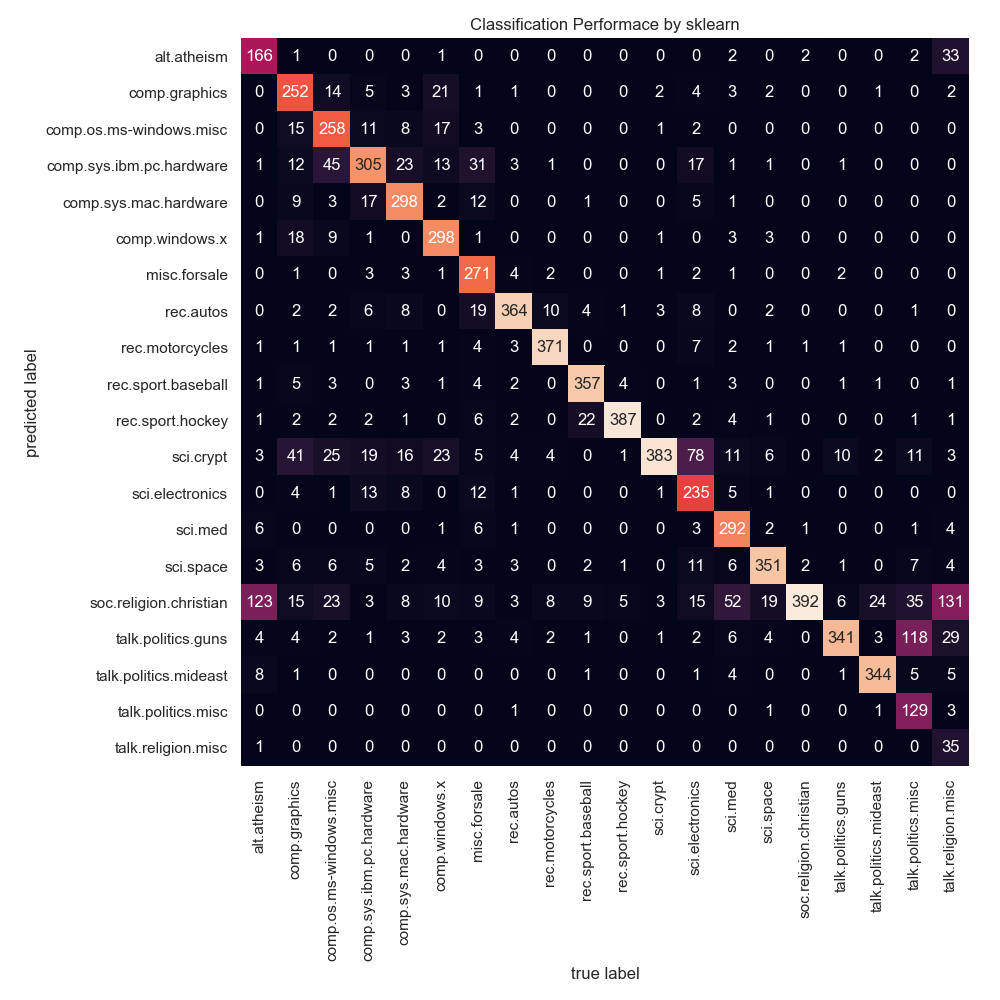
\includegraphics[width=2.5in, valign=t]{{naive_bayes/output/nbm_sklearn.png}}
        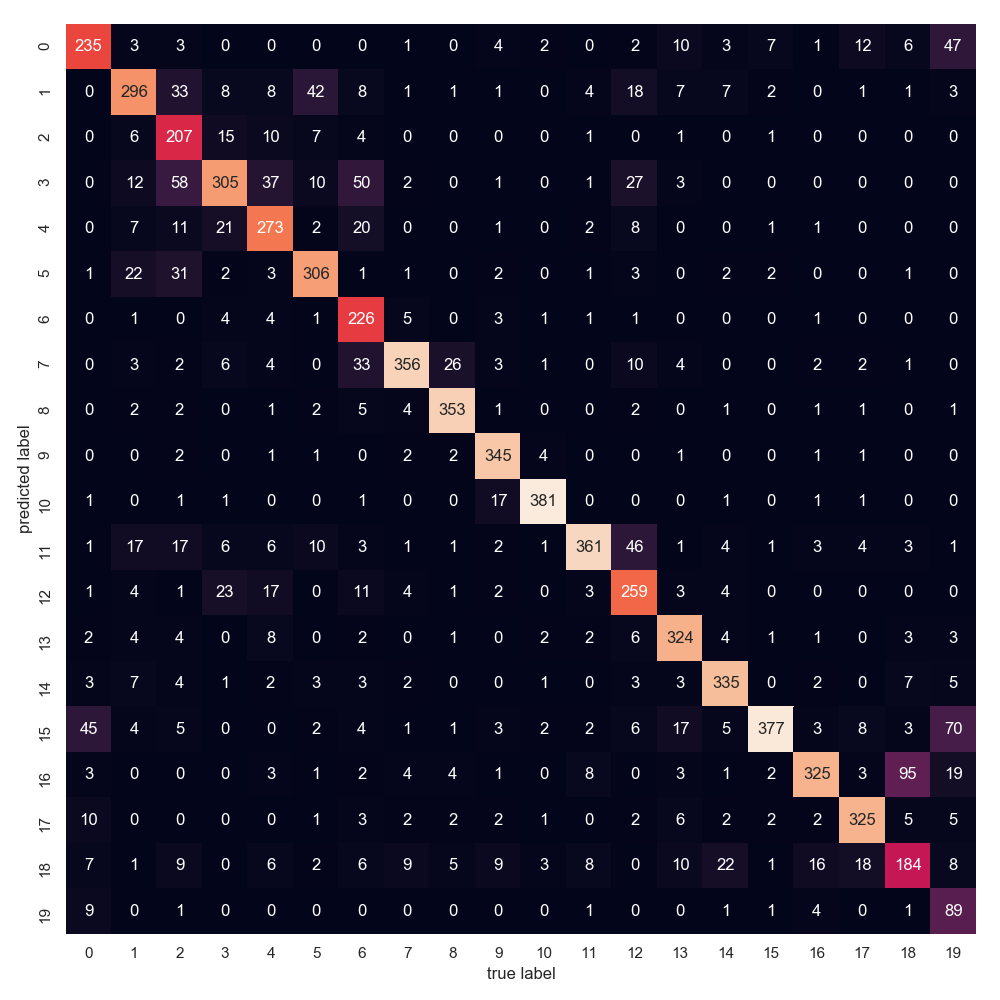
\includegraphics[width=2in, valign=t]{{naive_bayes/output/nbm_mine.png}}
    \end{center}
\end{figure}

\paragraph{b)}

Naive Bayes is a generative model. This is because it learns the actual probability distribution of words in
different document classes. It does not simply learn a decision boundary between the classes. Naive Bayes
is different from logistic regression because logistic regression can only separate data. Meanwhile, Naive
Bayes can generate data from the model it learns. A pro of Naive Bayes is that it is simple to understand
and train. Drawbacks include that it makes a very strong assumption that our document is a bag of words
that are independent of each other, and that it will not work very well when our data is imbalanced. If
a class in the training data does not contain a word, our classifier would incorrectly classify any document
of the class that does contain that word. This is solved with smoothing.

\section*{Problem 2}

\paragraph{a)}

The following tables show the most relevant words for each topic on each dataset.
\begin{center}
    \begin{tabular}{cccc}
        \multicolumn{4}{c}{Dataset 1} \\
        \hline
        Topic 1 & Topic 2 & Topic 3 & Topic 4\\
        \hline
        grand & luffy & crew & luffy\\
        sea & devil & pirates & pirates\\
        blue & fruit & island & haki\\
        island & user & luffy & piece\\
        dressrosa & fruits & straw & manga\\
        red & sea & grand & roger\\
        mountain & ace & robin & zou\\
        bur & crew & franky & captain\\
        half & water & hat & nami\\
        alliance & animals & government & sanji
    \end{tabular}
\end{center}
\begin{center}
    \begin{tabular}{cccc}
        \multicolumn{4}{c}{Dataset 2} \\
        \hline
        Topic 1 & Topic 2 & Topic 3 & Topic 4\\
        \hline
        bush & people & bank & percent\\
        percent & percent & soviet & people\\
        national & government & police & bush\\
        york & officials & company & president\\
        california & dukakis & oil & fire\\
        noriega & soviet & people & barry\\
        duracell & president & war & report\\
        police & central & roberts & fbi\\
        economic & administration & officers & rating\\
        president & expected & saudi & monday
    \end{tabular}
\end{center}

\paragraph{b)}

Yes, they generate probability distributions.

\paragraph{c)}

We need to manually select the number of topics, and it's hard to interpret how the results
come about. It can work on a lot of data but it seems to be repeating words.

\end{document}